\documentclass[11pt]{article}
\usepackage[margin=0.9in]{geometry}
\usepackage{amsmath,amssymb,booktabs,array,microtype,url,hyperref,tikz}
\usetikzlibrary{arrows.meta,positioning}
\usepackage[T1]{fontenc}
\usepackage{lmodern}
\hypersetup{
  colorlinks=true,
  linkcolor=black,
  citecolor=blue,
  urlcolor=blue,
  pdftitle={IEPP: Policy-Relative Canonical Continuation for Copyable AI Agents},
  pdfauthor={Woocheol Seo},
  pdfsubject={Registry-relative execution-lineage verification for copyable AI agents},
  pdfkeywords={AI agents, canonical continuation, execution lineage, rollback, fork, protocol security}
}
\newcommand{\iepp}{\textsc{IEPP}}
\newcommand{\ccg}{\textsc{CCG}}
\newcommand{\Hash}{\mathsf{H}}
\newcommand{\Accept}{\mathsf{Accept}}

\title{IEPP: Policy-Relative Canonical Continuation\\for Copyable AI Agents}
\author{Woocheol Seo\\Independent Researcher\\\texttt{iepp.protocol@gmail.com}\\\url{https://entropyproof.com}}
\date{September 2026}

\begin{document}
\maketitle

\begin{abstract}
Long-running AI agents can be copied, snapshotted, rolled back, migrated, and forked. A static identifier or signing key authenticates a credential holder, but does not show that one execution is the accepted continuation of a previously accepted execution. We call this the \emph{canonical-continuation problem} and present the Individual Entity Proof Protocol (\iepp), an early-stage protocol for registry-relative execution-lineage verification. \iepp{} binds a fresh challenge, monotonic counter, current canonical commitment, declared evidence, and enrolled signing key into an authenticated transition. An atomic registry accepts at most one successor of a canonical head. TRP~2.0 is a capability-indexed Canonical Continuation Game spanning observation through key-plus-state and registry compromise. A public L1 implementation accepted 50,000 valid transitions and recorded no false accepts in 10,000 trials each of replay, rollback/losing-fork, and signed-field substitution, no double accepts in 1,000 fork races, and no invariant violation in a bounded exploration of 1,063,623 states and 2,319,131 transitions. An ablation that removed both entropy fields likewise recorded no replay false accept in 10,000 trials and no double accept in 1,000 races, confirming that canonical serialization comes from freshness, predecessor agreement, and atomic head update rather than entropy. A declared entropy commitment remains a policy and audit hook; it does not certify unpredictability. Current-key-plus-state compromise and isolated registries remain explicit failure boundaries. The evidence supports only a narrow L1 single-registry software claim.
\end{abstract}

\section{Introduction}
AI agents increasingly retain memory, invoke tools, hold credentials, and act over long horizons. Yet their software, model weights, configuration, process state, and virtual machines remain copyable. If a signing key is also copied, two processes can produce valid signatures from the same enrolled authority. This creates a distinction that ordinary authentication does not resolve:
\begin{enumerate}
  \item \textbf{Credential identity:} does the presenter control an enrolled key or identifier?
  \item \textbf{Execution continuity:} is the presenter the next accepted continuation of the execution lineage previously recognized by a verifier?
\end{enumerate}

The second question appears after snapshots, rollbacks, concurrent replicas, migration, or compromise. Independent copies may diverge under different entropy or inputs, but divergence alone cannot decide which branch should be privileged. Canonicality requires an explicit acceptance rule and governance context.

We present the Individual Entity Proof Protocol (\iepp), a protocol for verifying execution lineage in copyable AI agents. Rather than equating identity with structural uniqueness, \iepp{} asks whether authenticated evidence advances a previously accepted trajectory under an explicit policy and registry view.

This paper makes four contributions:
\begin{itemize}
  \item it separates credential authentication, empirical branch divergence, and policy-relative canonical continuation;
  \item it specifies a domain-separated transition construction with challenge freshness, predecessor binding, monotonic counters, declared evidence hooks, and atomic single-successor acceptance;
  \item it defines TRP~2.0 as a capability-indexed Canonical Continuation Game, including explicit boundaries where L1 software protection fails; and
  \item it reports reproducible positive results together with negative controls, an entropy-field ablation, and a bounded single-host durability study.
\end{itemize}

We do \emph{not} claim consciousness, personhood, legal identity, physical uniqueness, a general reduction proving TRP hardness, or production readiness. We also do not claim that randomness or behavioral statistics reveal the canonical copy.

\section{IEPP Overview and Design Rationale}
\subsection{Motivating scenario and protocol objective}
Consider a long-running agent copied at some point into two processes with the same model, memory, configuration, and signing key. Both processes can pass ordinary credential authentication and signature verification. Credential possession alone therefore cannot determine which execution continues a previously accepted lineage.

IEPP does not attempt to determine metaphysical originality among copies. Its operational objective is narrower: under an explicit verification policy and registry view, determine which candidate succeeds the previously accepted state and is admitted as the next canonical state. This scope makes the protocol's decision boundary and trust assumptions explicit.

At each step, the verifier issues a challenge that can be used only once. A candidate binds the challenge, previously accepted state, next sequence number, and declared current-execution evidence into a signed transition. The registry verifies predecessor consistency, challenge freshness, sequence, signature, and policy conditions, then atomically records at most one successor. A later copy may still produce a cryptographically valid signature, but a consumed challenge or stale predecessor prevents its acceptance as the canonical successor.

\begin{figure}[t]
\centering
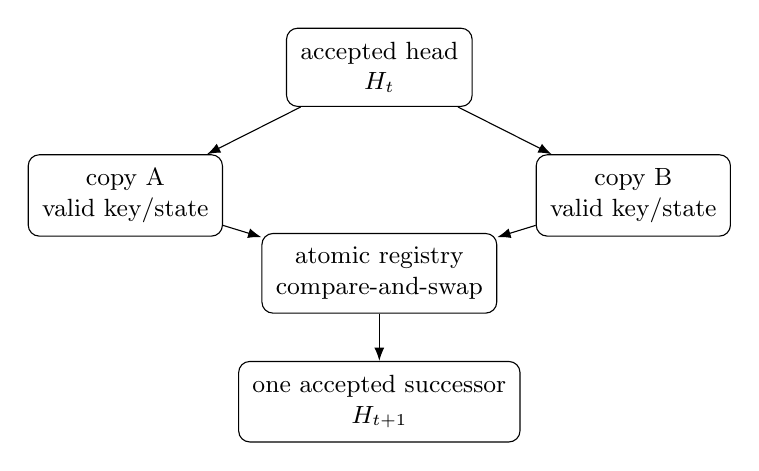
\begin{tikzpicture}[node distance=6mm and 8mm,>=Latex,every node/.style={font=\small},box/.style={draw,rounded corners,align=center,inner sep=5pt}]
\node[box] (head) {accepted head\\$H_t$};
\node[box,below left=of head] (a) {copy A\\valid key/state};
\node[box,below right=of head] (b) {copy B\\valid key/state};
\node[box,below=16mm of head] (reg) {atomic registry\\compare-and-swap};
\node[box,below=of reg] (next) {one accepted successor\\$H_{t+1}$};
\draw[->] (head) -- (a); \draw[->] (head) -- (b);
\draw[->] (a) -- (reg);
\draw[->] (b) -- (reg);
\draw[->] (reg) -- (next);
\end{tikzpicture}
\caption{Credential validity does not select a branch. Under one consistent registry view, the atomic head update accepts at most one successor; the other candidate becomes stale.}
\label{fig:fork}
\end{figure}

\subsection{Operational semantics and core concepts}
In this paper, \emph{canonical} means the one branch accepted under an explicit policy and registry view; it does not mean an objective or philosophical original. The \emph{registry} is a verification service that stores the current accepted head, counter, consumed challenges, and audit information. A \emph{transition} is the signed evidence submitted to move from one accepted state to the next. A \emph{commitment} is a hash that binds a value without necessarily disclosing it; a commitment alone does not certify that the value is truthful or high quality. \emph{Entropy} is variable runtime input from an allowed source. IEPP binds declared entropy into a transition, but does not claim that entropy alone proves identity or originality. A \emph{fork} consists of competing candidates derived from the same predecessor.

\subsection{Notation and domain separation}
Table~1 summarizes the notation used in the protocol definition. This specification defines three public domain-separation labels: $D_E$ is the literal ASCII byte sequence \texttt{IEPP-Entropy-v1}, $D_S$ is \texttt{IEPP-State-vNext-1}, and $D_X$ is \texttt{IEPP-Evidence-vNext-1}. They are neither variables nor values obtained from an earlier document, deployment, or secret configuration; an implementation inserts these exact bytes as hash inputs. Distinct labels prevent values created for different purposes from being silently interchanged. The \texttt{vNext-1} spellings are retained for compatibility with the evaluated public implementation; changing them would define a new wire profile and invalidate existing test vectors.

\begin{table}[ht]
\centering\small
\caption{Core notation.}
\begin{tabular}{p{0.18\textwidth}p{0.70\textwidth}}\toprule
Symbol & Meaning\\\midrule
$id$ & enrolled agent or entity identifier\\
$protocol$ & authenticated protocol-profile identifier\\
$domain$ & deployment or application scope fixed at enrollment\\
$t$ & monotonically increasing transition number\\
$H_t$ & registry's current canonical head at step $t$\\
$S_t$ & state commitment at step $t$\\
$E_t,EC_t$ & raw runtime entropy and its commitment\\
$source_t$ & declared entropy-source label checked by policy\\
$cid_t,nonce_t,expiry_t$ & challenge identifier, one-time nonce, and expiry\\
$R_t,A_t$ & optional runtime-state and platform-attestation commitments\\
$X_t,\sigma_t$ & transition-evidence body and its signature\\
$D_E,D_S,D_X$ & literal public domain-separation labels defined above\\
$key\_id,pk$ & enrolled signing-key identifier and public key\\
$\Hash$ & cryptographic hash function, SHA-256 in the reference profile\\
$\parallel$ & length-prefixed, order-preserving concatenation\\
$\Accept$ & registry decision after all policy checks succeed\\\bottomrule
\end{tabular}
\end{table}

For byte strings $x_1,\ldots,x_n$, the reference encoder computes
\begin{equation}
\Hash_D(x_1,\ldots,x_n)=\mathrm{SHA256}(\mathrm{u32}(|D|)\parallel D\parallel
\mathrm{u64}(|x_1|)\parallel x_1\parallel\cdots\parallel\mathrm{u64}(|x_n|)\parallel x_n),
\end{equation}
where integer lengths are unsigned big-endian values. Empty optional fields have length zero. This definition removes concatenation ambiguity; alternative profiles may use another injective canonical encoding if the profile identifier changes.

IEPP's conclusion is registry- and policy-relative. An isolated registry split or compromise of both the current key and state exceeds the present L1 guarantee. Stating these failure conditions is part of the threat model, rather than an exception hidden from the reader.

\section{Evolution of the Problem Formulation}
IEPP emerged through a sequence of testable formulations rather than from a single confirmed premise. An earlier IEPP whitepaper, v0.3, was released in the public project repository as a preliminary technical report. It investigated whether challenge-bound commitments and runtime entropy produced distinguishable execution trajectories~\cite{seo2026v03}. It reported immediate fork divergence in 100 of 100 runs and no successes in 50,000 attempts across five implemented cases: last-response replay, random-prior-response replay, challenge substitution, secret-guessing forgery, and seeded-PRNG imitation. However, the original--fork statistical score gap was only 0.015. These observations supported trajectory instrumentation but did not establish original-copy discrimination or a general security theorem.

The subsequent v0.4 whitepaper tested the statistical hypothesis more directly~\cite{seo2026v04}. Its reported original--fork score gap of $-0.047$ failed to identify a privileged original. This negative result changed the governing question: stochastic divergence and output resemblance could remain diagnostic signals, but neither could select successor authority. The project therefore moved from statistical ``original detection'' to policy-relative canonical lineage.

The v0.5 whitepaper then separated continuity measurement from application policy, registry behavior, migration, recovery, and deployment proposals~\cite{seo2026v05}. The current Core formulation subsequently narrowed the claim to authenticated, predecessor-bound transitions and atomic single-successor acceptance within a declared registry view. TRP~2.0 similarly replaces a broad reconstruction intuition with capability-indexed games and explicit failure boundaries.

This progression is methodologically important: the present protocol is partly the result of hypotheses that were rejected or restricted by experiment. The historical reports are cited as preliminary technical records, not as cumulative proof. A repository evidence map records the questions, results, superseded interpretations, and current reading order~\cite{seo2026evolution}.

\section{Problem and System Model}
\subsection{Canonical histories}
For an enrolled entity identifier $id$, let the accepted history through step $t$ be
\begin{equation}
  \mathcal{T}_{0:t}=(S_0,X_1,S_1,\ldots,X_t,S_t),
\end{equation}
where $S_t$ is a state commitment and $X_t$ is authenticated transition evidence. The canonical registry head is
\begin{equation}
  H_t=(id,t,S_t,key\_id,policy\_state).
\end{equation}
Two correctly signed candidates may fork from the same $S_t$. A candidate becomes canonical only after satisfying registry and policy rules. Thus ``validly produced'' and ``canonically accepted'' are distinct predicates.

\subsection{Threat question}
At a declared compromise boundary $t$, an adversary receives a view $V_t$. Depending on the evaluated profile, $V_t$ may include the public transcript, code and configuration, historical or current commitments, partial internal state, a process or VM snapshot, the signing key, entropy influence, verifier influence, or registry influence. The security question is whether the adversary can cause an \emph{unauthorized} future transition to be accepted as canonical under the claimed evidence level.

\subsection{Trust assumptions}
Every \iepp{} claim depends on explicit assumptions:
\begin{enumerate}
  \item hash and signature algorithms retain their conventional security properties;
  \item verifier challenges are fresh, entity-bound, and auditable;
  \item the registry advances a canonical head atomically or exposes equivocation;
  \item protected state is not modified undetectably at the claimed evidence level;
  \item entropy satisfies only its declared source profile; and
  \item enrollment, migration, recovery, and disputes are governed externally.
\end{enumerate}

\section{Protocol Construction}
\subsection{Enrollment and entropy commitment}
Enrollment records $(id,domain,key\_id,pk,S_0,policy)$. Raw runtime entropy $E_t$ is not disclosed. The prover instead computes
\begin{equation}
  EC_t=\Hash_{D_E}(E_t).
\end{equation}
This commitment can hide the sampled bytes under the hash assumption and permit equality tests. It does not prove unpredictability, physical origin, or source integrity.

\subsection{Authenticated transition}
For a fresh challenge $(cid_t,nonce_t,expiry_t)$ and monotonic counter $t$, let $R_t$ and $A_t$ denote the optional runtime and attestation commitments. The prover computes
\begin{align}
  S_t=\Hash_{D_S}(&id,domain,t,S_{t-1},cid_t,nonce_t,\nonumber\\
                  &EC_t,source_t,R_t,A_t).
\end{align}
The complete transition body and signature are
\begin{align}
X_t={}&(protocol,id,domain,t,S_{t-1},S_t,cid_t,nonce_t,expiry_t,\nonumber\\
      &EC_t,source_t,R_t,A_t,key\_id),\\
B_t={}&\Hash_{D_X}(X_t),\qquad \sigma_t=\mathrm{Sign}_{sk}(B_t).
\end{align}
Here $\Hash_{D_X}(X_t)$ means that the ordered fields of $X_t$ are encoded separately by the canonical encoder above, not that an ambiguous textual tuple is hashed. SHA-256 and Ed25519 are reference-profile choices, not essential to the state-machine semantics.

\begin{figure}[t]
\centering
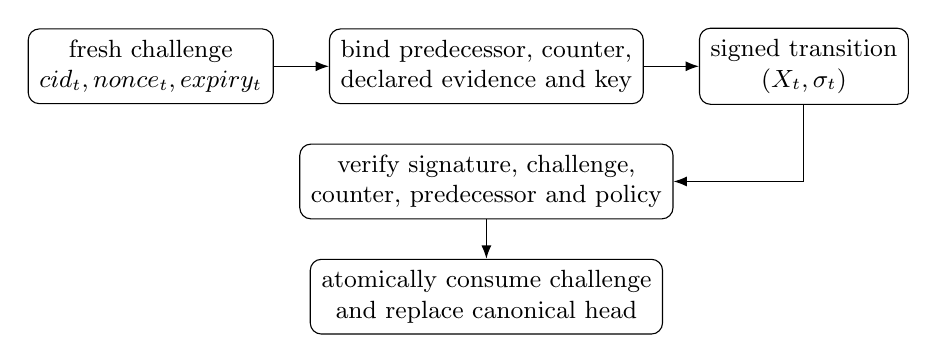
\begin{tikzpicture}[node distance=5mm and 7mm,>=Latex,every node/.style={font=\small},box/.style={draw,rounded corners,align=center,inner sep=4pt}]
\node[box] (challenge) {fresh challenge\\$cid_t,nonce_t,expiry_t$};
\node[box,right=of challenge] (build) {bind predecessor, counter,\\declared evidence and key};
\node[box,right=of build] (signed) {signed transition\\$(X_t,\sigma_t)$};
\node[box,below=of build] (checks) {verify signature, challenge,\\counter, predecessor and policy};
\node[box,below=of checks] (cas) {atomically consume challenge\\and replace canonical head};
\draw[->] (challenge) -- (build); \draw[->] (build) -- (signed);
\draw[->] (signed) |- (checks); \draw[->] (checks) -- (cas);
\end{tikzpicture}
\caption{Transition construction and registry decision path. Entropy is a declared evidence hook; single-successor selection occurs at the final atomic update.}
\label{fig:transition}
\end{figure}

\subsection{Procedures}
\paragraph{ProveTransition.} Given the enrolled secret key, current head, fresh entity-bound challenge, declared evidence, and optional commitments, the prover (1) checks challenge addressing and expiry, (2) computes $EC_t$ and $S_t$, (3) constructs $X_t$ with counter $t$, (4) signs $B_t$, and (5) returns $(X_t,\sigma_t)$. Raw $E_t$ is retained unless an audit policy later requires opening the commitment.

\paragraph{VerifyAndAdvance.} The registry parses $X_t$ and requires protocol, entity, domain, and key identifiers to match enrollment. It verifies $\sigma_t$; challenge ownership, nonce, expiry, and non-consumption; $t=H_{t-1}.t+1$; $S_{t-1}=H_{t-1}.S$; policy constraints; and recomputed $S_t$. In one compare-and-swap transaction it aborts if the stored head changed, otherwise consumes the challenge, writes $H_t$, and appends the evidence to the audit chain. Any failed precondition rejects without advancing the head.

\subsection{Single-successor acceptance}
Cryptographic validity alone does not make a transition canonical: a validly produced candidate becomes canonically accepted only through the atomic registry decision above. The resulting invariant is

\begin{equation}
  \forall H_t:\quad \#\{S_{t+1}:\Accept(H_t,S_{t+1})\}\leq 1
  \label{eq:single-successor}
\end{equation}
within one consistent registry view. Competing successors may remain auditable branches, but only the committed successor is canonical.

\subsection{Audit, equivocation, and migration}
Accepted transitions extend a hash-chained audit root. A registry can sign checkpoints containing its identifier, sequence, entity, counter, canonical head, and audit root. Conflicting signed checkpoints at the same logical position become evidence of equivocation when compared. Detection still requires gossip, a quorum, transparency logging, or an external anchor; isolated verifiers cannot detect a split view.

Key migration binds the current head and counter, old and new key identifiers, the new public key, and a fresh challenge. The reference profile requires both old and new keys to sign. Recovery without the old key is a separate, auditable policy event rather than an ordinary continuation.

\section{TRP 2.0: Canonical Continuation Game}
Earlier formulations of the Trajectory Reconstruction Problem asked whether a clone could reconstruct an execution trajectory. That wording can conflate stochastic divergence with authorization. TRP~2.0 instead evaluates unauthorized canonical continuation.

The challenger enrolls an entity, advances it to $H_t$, and releases the profile-defined view $V_t$. For attack budget $q$, adversary $\mathcal{A}$ wins when
\begin{equation}
  \Accept(candidate)=1
\end{equation}
and the candidate is unauthorized by the evaluated policy. We denote this experiment the Canonical Continuation Game (\ccg) and write
\begin{equation}
  \mathrm{Adv}^{\ccg}_{\mathcal{A}}(t,q,profile)=\Pr[Win=1].
\end{equation}
``Unauthorized'' must be policy-defined. In particular, stolen current authority is not mislabeled as signature forgery.

\begin{table}[t]
\centering
\caption{TRP 2.0 capability hierarchy.}
\label{tab:capabilities}
\small
\begin{tabular}{p{0.07\columnwidth}p{0.81\columnwidth}}
\toprule
Class & Capability and evaluated question\\
\midrule
A0 & Public transcript: replay or forgery from observation?\\
A1 & Code/configuration copy: silent canonical continuation?\\
A2 & Partial-state leakage: what continuation advantage results?\\
A3 & Process/VM snapshot: double acceptance or replacement?\\
A4 & Entropy influence: undetected evidence overclaim?\\
A5 & Current key plus state: can the clone win the next race?\\
A6 & Host, verifier, or registry control: what stronger mechanism remains?\\
\bottomrule
\end{tabular}
\end{table}

Required properties include replay resistance, predecessor continuity, fork serialization, rollback resistance, evidence-level honesty, and---when claimed---equivocation detectability. Results at one capability class do not generalize to a stronger class. A5 is an expected failure boundary for the present L1 profile.

\section{Implementation and Evaluation}
\subsection{Reference profile}
The public Python implementation uses SHA-256, Ed25519, entity- and domain-bound one-time challenges, monotonic counters, authenticated evidence, an atomic in-memory registry, signed checkpoints, dual-signature migration, and a SQLite WAL/FULL-synchronous compare-and-swap store. The evaluated \texttt{reference/iepp\_vnext} artifact is pinned by the following Git tree:
\begin{center}\small\ttfamily d6cd7f7f4b48c6a2a020ae3a240041b306b779ed\end{center}
From that directory, the principal reproduction commands are:
\begin{quote}\small\ttfamily
python run\_trp2\_ci.py\\
python -m unittest discover -s tests -v\\
python entropy\_ablation.py
\end{quote}
All reported results are L1 software evidence.

\subsection{Research questions and metrics}
We test whether valid sequential transitions are accepted; replay, stale-predecessor, rollback, signed-field substitution, and losing forks are rejected; concurrent successors are serialized; durable state survives tested restart and injected-fault cases; and the bounded model preserves Eq.~\ref{eq:single-successor}. The primary metric is unauthorized canonical acceptance. First divergence and output similarity are diagnostics, not security proofs.

\subsection{Reproducible results}
Table~\ref{tab:results} reports the fixed public experiment budgets. When zero adverse events are observed in $n$ independent Bernoulli trials, the displayed 95\% upper event-rate bound uses the rule of three, $3/n$. This is a finite-sample statistical statement, not a cryptographic security bound.

\begin{table}[t]
\centering
\caption{Reproducible L1 results. Zero observed events do not imply an unconditional zero probability.}
\label{tab:results}
\small
\begin{tabular}{>{\raggedright\arraybackslash}p{0.18\textwidth}p{0.13\textwidth}p{0.15\textwidth}>{\raggedright\arraybackslash}p{0.40\textwidth}}
\toprule
Experiment & Budget & Adverse events & Interpretation\\
\midrule
Valid transitions & 50,000 & 0 rejects & Reference functional path\\
Replay & 10,000 & 0 false accepts & 95\% upper event-rate bound $\approx0.03\%$\\
Rollback / losing fork & 10,000 & 0 false accepts & Same finite-sample bound\\
Field substitution & 10,000 & 0 false accepts & Same finite-sample bound\\
Concurrent forks & 1,000 & 0 double accepts & 95\% upper event-rate bound $\approx0.3\%$\\
Shuffled retry & 2,000 & 0 final failures & Eventual ordered acceptance in tested model\\
Duplicate delivery & 2,000 & 0 false accepts & Every duplicate rejected as replay\\
Bounded search & 1,063,623 states & 0 violations & 2,319,131 abstract transitions explored\\
Historical divergence & 100 runs & 0 failures & All 100 diverged; diagnostic only, not canonicality evidence\\
Historical attacks & 50,000 trials & 0 successes & Limited to the five v0.3 cases listed in Section~3\\
\bottomrule
\end{tabular}
\end{table}

On the recorded single-process Linux host, mean challenge issuance, prover transition/signature, registry verification/advance, and checkpoint operations were 0.0030, 0.0430, 0.1189, and 0.0344 ms. The 50,000-step loop processed approximately 6,050 transitions/s. These figures exclude networks, consensus, distributed durable stores, and attestation.

\subsection{Single-host durability observation}
A supplemental SQLite research prototype executed deterministic F00--F12 cases at transaction and recovery boundaries. In those cases, no pre-commit fault left a partial acceptance; commit-response loss followed by exact retry did not advance the state twice; exactly one of two successors from one predecessor committed; checkpoint regeneration after restart succeeded; and simulated corruption failed closed rather than silently creating a new genesis. An internally consistent rollback of the complete database was \emph{not} locally detectable. These observations are bounded to the tested implementation and deterministic schedules; they do not establish crash consistency across operating systems, filesystems, storage hardware, process-kill schedules, or distributed registries.

\subsection{Required negative controls}
Four negative results define the actual boundary:
\begin{enumerate}
  \item \textbf{Predictable entropy.} One thousand unique counter-derived values were accepted when policy labeled the source as allowed. A commitment cannot certify entropy quality.
  \item \textbf{Key-plus-state compromise.} A clone holding the current state and valid signing key was accepted when it submitted first; the legitimate branch lost that race.
  \item \textbf{Registry split view.} Two isolated registries accepted different successors. Conflict became detectable only after their signed checkpoints were compared.
  \item \textbf{Statistical clone-separation failure.} Historical experiments produced original--fork score gaps of 0.015 and $-0.047$, which did not identify a canonical clone. Registry-relative acceptance therefore replaces statistical resemblance as the decision mechanism.
\end{enumerate}

\subsection{Entropy-field ablation}
To isolate the source of canonical serialization, we evaluated a comparison variant that removes both $EC_t$ and $source_t$ while retaining the registered key, one-time challenge, predecessor, monotonic counter, signature, and atomic head update. Table~\ref{tab:ablation} shows that the tested replay and concurrent-fork outcomes were unchanged. This does not make entropy useless: a declared commitment can support later equality checks, source policy, audit, and stronger platform profiles. It does establish that entropy is not the L1 mechanism that chooses the canonical successor.

\begin{table}[t]
\centering
\caption{Entropy-field ablation. Results are bounded observations, not universal probability claims.}
\label{tab:ablation}
\small
\begin{tabular}{p{0.27\textwidth}p{0.27\textwidth}p{0.27\textwidth}}
\toprule
Variant & Replay trials & Concurrent fork races\\
\midrule
Full L1 profile & 0 false accepts / 10,000 & 0 double accepts / 1,000\\
No entropy fields & 0 false accepts / 10,000 & 0 double accepts / 1,000\\
\bottomrule
\end{tabular}
\end{table}

\section{Evidence Levels}
\begin{table}[t]
\centering
\caption{Claims must not exceed deployment evidence.}
\label{tab:levels}
\small
\begin{tabular}{p{0.10\columnwidth}p{0.78\columnwidth}}
\toprule
Level & Trust basis\\
\midrule
L1 & Software key/state, declared OS entropy, authenticated transcript, single registry\\
L2 & Isolated key/state plus platform attestation\\
L3 & Witnessed/quorum registry or transparency gossip\\
L4 & Evaluated hardware identity plus PUF or protected physical entropy\\
\bottomrule
\end{tabular}
\end{table}
\iepp{} does not replace TPMs, TEEs, secure elements, PUFs, transparency systems, or consensus. It provides state-machine semantics into which such mechanisms may be bound. L2--L4 claims require separate implementations and evaluations.

\section{Related Work}
AgentDID combines decentralized identifiers, verifiable credentials, and challenge--response evidence for agent authentication and runtime-condition validation~\cite{xu2026agentdid}. BlockA2A combines DIDs, blockchain anchoring, and policy enforcement for agent-to-agent authenticity, auditability, and access control~\cite{zou2025blocka2a}. SAGA focuses on identity, authorization, lifecycle control, and governance for agentic systems~\cite{syros2025saga}. These systems establish or govern agent authority; \iepp{} isolates the narrower question of whether a presentation advances one accepted execution lineage.

FP-Agent shows that browser and behavioral features can classify browsing agents, while also finding limits when agents share browser fingerprints~\cite{wang2026fpagent}. Such fingerprinting is useful for detection and traffic control, but classification evidence does not serialize successor authority. A recent agent-security survey identifies long-lived state, credentials, tools, and cross-component interactions as a distinct systems-security surface~\cite{kim2026landscape}; \iepp{} supplies one explicit continuity primitive within that broader surface.

Proof-of-Continuity studies causal, non-expansive propagation of authority across execution steps~\cite{gallo2026continuity}. Its authorization-chain question is complementary to \iepp{}'s canonical-successor question. W3C DIDs and Verifiable Credentials define interoperable identifiers and tamper-evident claims~\cite{w3cdid,w3cvc}. C2PA binds provenance assertions to content assets~\cite{c2pa}. \iepp{} instead concerns a continuing executor, although an IEPP checkpoint could be carried in a credential or provenance assertion.

Remote attestation provides an architecture for conveying and appraising evidence about an attester's operating state~\cite{rfc9334}; TPM~2.0 supplies protected platform primitives that can support stronger profiles~\cite{tcgtpm}; Certificate Transparency illustrates publicly auditable append-only logging and split-view concerns~\cite{rfc9162}; and Raft illustrates consensus over a replicated log~\cite{ongaro2014raft}. \iepp{} deliberately does not reimplement attestation, hardware roots, transparency, or consensus. Its contribution is the explicit composition point among authenticated transition evidence, evolving state, canonical acceptance, and evidence-level claims. Accordingly, Eq.~\ref{eq:single-successor} is a single-registry invariant, not a distributed-consensus result.

\section{Limitations and Open Research}
The present study is software-only and authored by the protocol proposer. It lacks independent reproduction, peer review, unbounded formal verification, and real adversarial deployment. Conventional hash and signature assumptions are used, but no reduction proves a general TRP-hardness theorem. Eq.~\ref{eq:single-successor} is scoped to one consistent registry view and does not survive partition without a witnessed-registry mechanism. Current state plus signing-key compromise wins at L1. Entropy-health policy remains incomplete, and an entropy commitment is not attestation. Privacy leakage from repeated lineage checkpoints has not been analyzed.

Priority experiments are hypervisor-level VM snapshot/restore; partial-state leakage sweeps; entropy freeze, repetition, bias, substitution, and unavailability; post-compromise key/state refresh and revocation; split-view detection latency under gossip, quorum, or anchoring; and hardware-backed evaluation on TPM, TEE, or secure-element platforms. Authorized migration, recovery authority, and legal responsibility remain governance questions.

\section{Conclusion}
Copyable agents require a distinction between authenticating a credential and accepting an execution continuation. \iepp{} makes this distinction explicit through challenge-bound, predecessor-bound, authenticated transitions and an atomic canonical-head rule. TRP~2.0 turns a broad originality intuition into capability-indexed games with measurable success conditions and explicit compromise boundaries.

Current evidence supports only a narrow L1 conclusion: under the tested single-registry assumptions, the reference implementation accepted valid transitions and rejected the evaluated replay, rollback, substitution, and losing-fork attempts, while deterministic single-host durability cases preserved atomicity at the tested fault points. Negative controls show why stronger conclusions would be unjustified. The resulting research direction is not ``randomness proves identity,'' but that evolving evidence, protected authority, and canonical policy can make execution-lineage continuity an explicit, testable component of AI-agent trust.

\section*{Artifact Availability}
Source code, specifications, tests, fixed result artifacts, and reproduction commands are available at \url{https://github.com/swc8121-alt/iepp}. The evaluated implementation is identified by the pinned Git tree in Section~7.1. Historical whitepapers are available at \url{https://entropyproof.com}.

\bibliographystyle{plain}
\bibliography{references}
\end{document}
